% !TEX root =main.tex
We illustrate our technique on a two-dimensional switched system with $4$ modes. We fix the condifence level, $\beta = 0.92$ and compute both upper and lower bounds on JSR for $N:=15+50k,\, k \in\{0, \ldots, 10\}.$ We demonstrate the performance of our algorithm 


We run our algorithm $10$ times and taking the average value for the lower bound, $\delta$, and the upper bound, we obtain the following plots.


\begin{figure}

\begin{center}
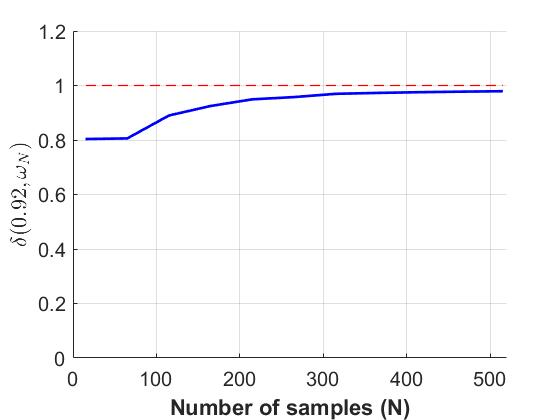
\includegraphics[scale=0.35]{delta1.jpg}
\caption{Evolution of $\delta$ along $N$.}
\end{center}
\end{figure}


\begin{figure}
\begin{center}
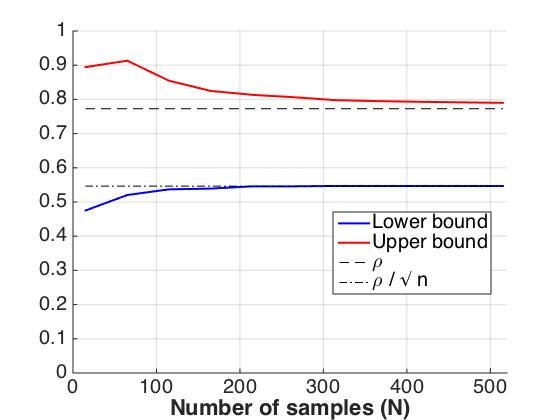
\includegraphics[scale=0.35]{bounds1.jpg}
\caption{Evolution of the bounds along $N$.}
\end{center}
\end{figure}

We observe that $\delta$ converges to $1$, the upper-bound converges to $\rho$, the value of the JSR, and the lower-bound converges to the value of the JSR divided by $\sqrt{n}$.

We then test our algorithm with a system in dimension $4$, with $5$ modes and JSR equal to $0.7929$. We observe a slower convergence of the values, even with more points in our sampling.
[to add plots here, but they are not super nice: we do not see the convergence to $1$ of $\delta$: even after $10 000$ points, $\delta$ is below $0.85$].

Finally, we generate $10000$ cases with systems of dimension between $2$ and $7$, number of modes $m$ between $2$ and $5$, and size of samples $N$ between $30$ and $800$. We take $\beta = 0.92$ and we test if the upper bound computed is greater than the actual JSR of the system. We get $xxx$ positive tests, giving us a probability of having an upper bound equal to $xxx$. 



